%Search time
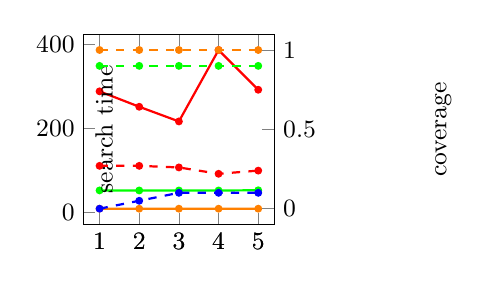
\begin{tikzpicture}
\small
    \begin{axis}[
    width = 4cm,
    height= 4cm,
    enlarge x limits = 0.1,
    enlarge y limits = 0.1,
    legend columns=3,
    legend style={at={(0.05,-0.3)},anchor=west},
    xmax = 5,
    xtick={1,2,3,4,5},
    xmin = 1,
	ylabel= search time,
	y label style={at={(0.2,0.5)}},
	axis y line*=left,
]

%blocksworld search time
\addplot[thick, blue, mark=*,
mark options={scale=0.5,solid},
]
        plot coordinates {
        };

%nomystery search time
\addplot[thick, red, mark=*,
mark options={scale=0.5,solid},
]
        plot coordinates {
			(1, 287.78)
			(2, 251.07)
			(3, 216.08)
			(4, 386.22)
			(5, 291.53)
        };

%tpp search time
\addplot[thick, green, mark=*, mark options={scale=0.5,solid},
]
        plot coordinates {
			(1, 51.76)
			(2, 51.65)
			(3, 51.64)
			(4, 51.66)
			(5, 52.11)
        };


%rovers search time
\addplot[thick, orange, mark=*, mark options={scale=0.5,solid},
]
        plot coordinates {
			(1, 8.24)
			(2, 8.25)
			(3, 8.28)
			(4, 8.25)
			(5, 8.25)
        };
\end{axis}

\begin{axis}[
    width = 4cm,
    height= 4cm,
    enlarge x limits = 0.1,
    enlarge y limits = 0.1,
    legend columns=3,
    legend style={at={(0.05,-0.3)},anchor=west},
    xmax = 5,
    xtick={1,2,3,4,5},
    xmin = 1,
	axis y line*=right,
	ylabel= coverage,
	y label style={at={(1.8,0.5)}},
	ytick={0,0.5,1},
	ymin=0,
	ymax=1,
]

%coverage blocksworld
\addplot[thick, blue, dashed, mark=*,
mark options={scale=0.5,solid},
]
        plot coordinates {
			(1, 0.0)
			(2, 0.05)
			(3, 0.1)
			(4, 0.1)
			(5, 0.1)
        };

%coverage nomystery
\addplot[thick, red, dashed, mark=*,
mark options={scale=0.5,solid},
]
        plot coordinates {
			(1, 0.27)
			(2, 0.27)
			(3, 0.26)
			(4, 0.22)
			(5, 0.24)
        };

%tpp coverage
\addplot[thick, green, dashed, mark=*, mark options={scale=0.5,solid},
]
        plot coordinates {
			(1, 0.9)
			(2, 0.9)
			(3, 0.9)
			(4, 0.9)
			(5, 0.9)
        };

%rovers coverage
\addplot[thick, orange, dashed, mark=*, mark options={scale=0.5,solid},
]
        plot coordinates {
			(1, 1.0)
			(2, 1.0)
			(3, 1.0)
			(4, 1.0)
			(5, 1.0)
        };

    \end{axis}


\end{tikzpicture}
%MUGS
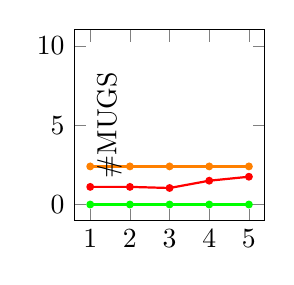
\begin{tikzpicture}

    \begin{axis}[
	%title = \#MUGS,
    width = 4cm,
    height= 4cm,
    enlarge x limits = 0.1,
    enlarge y limits = 0.1,
    legend columns=3,
    legend style={at={(0.05,-0.3)},anchor=west},
    xmax = 5,
    xmin = 1,
    xtick={1,2,3,4,5},
    ytick={0,5,10},
	ymin=0,
	ymax=10,
	ylabel= \#MUGS,
	y label style={at={(0.3,0.5)}},
]

%MUGS blocksworld
\addplot[thick, blue, mark=*,
mark options={scale=0.5,solid},
]
        plot coordinates {

        };

%MUGS nomystery
\addplot[thick, red, mark=*,
mark options={scale=0.5,solid},
]
        plot coordinates {
			(1, 1.11)
			(2, 1.11)
			(3, 1.04)
			(4, 1.5)
			(5, 1.75)
        };


%MUGS TPP
\addplot[thick, green, mark=*, mark options={scale=0.5,solid},
]
        plot coordinates {
			(1, 0.0)
			(2, 0.0)
			(3, 0.0)
			(4, 0.0)
			(5, 0.0)
        };

%MUGS rovers
\addplot[thick, orange, mark=*, mark options={scale=0.5,solid},
]
        plot coordinates {
			(1, 2.4)
			(2, 2.4)
			(3, 2.4)
			(4, 2.4)
			(5, 2.4)
        };
\end{axis}
\end{tikzpicture}


